%\documentclass{beamer}
% Aspect ratio
\documentclass[aspectratio=43,11pt]{beamer}
% Aspect ratio:
% 610 => 16:10 
% 169 => 16:9
% 149 => 14:9
%  54 => 5:4
%  43 => 4:3 Default
%  32 => 3:2

% Font size
% 8pt, 9pt, 10pt, 11pt (default), 12pt, 14pt, 17pt, 20pt

%\usefonttheme{default}
% structurebold
% structurebolditalic
% structuresmallcapsserif
% structureitalicsserif
% serif
% default. 

% Opciones de lenguaje usando polyglossia (defino dos para este documento)
\usepackage{polyglossia}
\setmainlanguage{spanish}
\setotherlanguage[variant=american]{english}
\usepackage{amssymb} % Los simbolos el los conjuntos numéricos

% El sistema de bibliografá es Biber (no necesitas BibTeX)
\usepackage[
  backend=biber
]{biblatex}
\addbibresource{biblio.bib}

\usepackage{graphicx} % Incluir imágenes
\usepackage{subcaption} % Poder usar subfiguras
% Para presentaciones usualmente no necestiamos la primer parte del caption
\captionsetup[figure]{labelformat=empty}
\captionsetup[table]{labelformat=empty}
% Tablas con estilo profesional
\usepackage{booktabs}

% Para usar varias columnas
\usepackage{multicol}

% Para poner algortmos en pseudo código
\usepackage{algpseudocode}
\usepackage{algorithm} %Ambiente flotante para los algoritmos
%Make the comments similar to cpp
%\algrenewcommand{\algorithmiccomment}[1]{\hskip3em$//$ #1}
%El paquete algorithm, no tiene traduccion automatica
\floatname{algorithm}{Algoritmo}
\renewcommand{\algorithmicrequire}{\textbf{Entradas:}}
\renewcommand{\algorithmicensure}{\textbf{Salidas:}}
\renewcommand{\listalgorithmname}{Índice de algoritmos}

\usepackage[newfloat=true]{minted} %Para insertar código fuente en algún lenguaje de programación
% Requiere que comiples usando:
% $xelatex -shell-escape input.tex

% Configuracion del entorno minted para poner código fuente
\DeclareCaptionFormat{mitedFormat}{%
    \textbf{#1#2}#3}
\DeclareCaptionStyle{minetdStyle}{skip=0cm,width=.85\textwidth,justification=centering,
  font=footnotesize,singlelinecheck=off,format=mitedFormat,labelsep=space}
\newenvironment{mintedCode}{\captionsetup{type=listing,style=minetdStyle}}{}

\usepackage{dirtytalk} %For using qutation marks (usa comillas in spanish)

% Cambia el nombre de la etiqueta. Afecta a todos los codigos minted del codumento
%\SetupFloatingEnvironment{listing}{name=Código}
\captionsetup[listing]{labelformat=empty}
% Opciones de minted para el lenguaje C++
\setminted[cpp]{frame=lines,framesep=0.25cm,baselinestretch=1,fontsize=\scriptsize,breaklines}
% Cuando lo hagas dentro de un parrafo el tamaño de fuente debe ser normal
\setmintedinline[cpp]{fontsize=auto}

\usetheme{default}

% Crear un comando con el nombre de la UNAM
\newcommand{\unam}{
  \bfseries
  \normalsize{Universidad Nacional Autónoma de México}
}

% Crear un comando para el email
\newcommand{\email}[1]{
    \texttt{
      \href{mailto:#1}{#1}
    }
}

%Information to be included in the title page:
\title[La revolución]{Mis años en la Revolución Mexicana}
\subtitle{Una historia personal}
\author[Pancho Villa]{José Doroteo Arango Arámbula}
\institute[FES Acatlán]{
%     email for contact
    \normalsize{\email{panchovilla@unam.mx}}
%    university name
%    \unam
}
\date
{Teoria de Gráficas, 2021-II}
\titlegraphic{
\includegraphics[width=1.7cm]{img/escudo-a}}

% Logo appears in all slides not only title
%\logo{
\includegraphics[height=1cm]{img/escudo-a}}

%Redefinimos algunos enviroments en español
\newtheorem{thm}{Teorema:}
\newtheorem{lem}{Lema:}
\newtheorem{mydef}{Definición:}
\newtheorem{obs}{Observación:}
\newtheorem{prop}{Proposición:}
\newtheorem{cor}{Corolario:}

\usetheme{Frankfurt}
\useinnertheme{circles}
\usecolortheme{orchid}
% Necesito redefinir smothbars para poder quitar las sombras abajo
\useoutertheme{smoothbars}

% Definicion de colores especiales
\definecolor{light_blue}{RGB}{4, 163, 198}
\definecolor{azul_unam}{RGB}{0, 43, 122}
\definecolor{dorado_unam}{RGB}{187, 136, 0} % 0.65, 0.53 0
\definecolor{amarillo_quemado}{RGB}{212, 180, 21}
\definecolor{light_gray}{RGB}{245, 245, 245}
\definecolor{light_golden}{RGB}{255, 245, 230} % 0.85, 0.73, 0.2 

% Quitar la sombra entre las secciones y los titulos
\makeatletter
\AtBeginDocument{
\pgfdeclareverticalshading{beamer@barshade}{\the\paperwidth}{%
         color(0ex)=(azul_unam);%
         color(0.5ex)=(section in head/foot.bg);%
         color(4ex)=(section in head/foot.bg)%
       }
}
\makeatother

\setbeamercolor{title}{fg=azul_unam,bg=dorado_unam}
\setbeamercolor{section in head/foot}{fg=dorado_unam,bg=azul_unam}
\setbeamercolor{frametitle}{fg=azul_unam,bg=dorado_unam}

\setbeamertemplate{blocks}[rounded][shadow=false]
% Disable shading between block title and block content
\makeatletter
\pgfdeclareverticalshading[lower.bg,upper.bg]{bmb@transition}{200cm}{color(0pt)=(lower.bg); color(4pt)=(lower.bg); color(4pt)=(upper.bg)}
\makeatother

\setbeamercolor{block title}{bg=dorado_unam,fg=azul_unam}
\setbeamercolor{block body}{bg=light_golden,fg=black}

% Quitar el redondeado de los slides con titulo
\setbeamertemplate{frametitle}[default][colsep=-4bp,rounded=false,shadow=false]
% Pongo linkcolor vacio para que los links internos no tengan color
% Solo los links externos tienen color
\hypersetup{colorlinks,linkcolor=,urlcolor=azul_unam}

\usepackage{csquotes} % Por que si no esta presnte AQUI polyglosia tira un warning

\begin{document}

% El contenido de la presentacion esta en este otro archivo
% Primer slide contiene el título
\begin{frame}{}
    \maketitle
\end{frame}

% Segundo slide el índice
\begin{frame}{Agenda}
    \begin{multicols}{2}
        \tableofcontents
    \end{multicols}
\end{frame}

\section{Antecedentes}
 \begin{frame}{¿Para que sirve?}
     Esta plantilla puede servir para:
     \begin{itemize}
         \item Presentar en una conferencia o evento
         \item Donde hay varios ponentes
         \item No todo mundo te conoce.
     \end{itemize}
     
     \vspace{0.4cm} % Insertar espacio vertical

     Para utilizar esta plantilla debes tener
     \begin{enumerate}
         \item Conocimientos mínimos de \LaTeX{}
         \item Leer el código fuente y el pdf al mismo tiempo
         \item Leer el la \href{https://github.com/nemediano/latexPlantillaUnam/tree/main/Conferencia}{documentación} del repositorio de la plantilla
     \end{enumerate}

     \vspace{0.2cm}

 \end{frame}

\subsection{Formato básico} 
\begin{frame}{Usando columnas}
\begin{columns}
\column[t]{0.5\textwidth}
     Esta es la primer columna
     \begin{itemize}
         \item Un poco de texto
         \item Un poco mas de texto
         \item El último texto
     \end{itemize}
\column[t]{0.5\textwidth}
     Segunda columna, nótese que están alineadas hacia arriba
     \begin{enumerate}
         \item Primer punto
         \item Segundo punto
         \item Tercer punto
     \end{enumerate}
\end{columns}
\end{frame}

\begin{frame}{Tipos de texto}
  \begin{itemize}
    \item En negritas (bf):  \textbf{Texto de ejemplo}
    \item En italicas (it) \textit{Texto de ejemplo}
    \item En slanted (sl) \textsl{Texto de ejemplo}
    \item En tipo de letra romana (rm) \textrm{Texto de ejemplo}
    \item En tipo de fuente san serif (sf) \textsf{Texto de ejemplo}
    \item En tipo de terminal (tt) \texttt{Texto de ejemplo}
    \item En color \textcolor{orange}{Texto de ejemplo}
    \item En alerta \alert{Texto de ejemplo}
    \item En estructura \structure{Texto de ejemplo}
  \end{itemize}
\end{frame}

\subsection{Añadir elementos}
\begin{frame}{Una imagen desde un archivo}
\begin{figure}[htb]
  \centering
  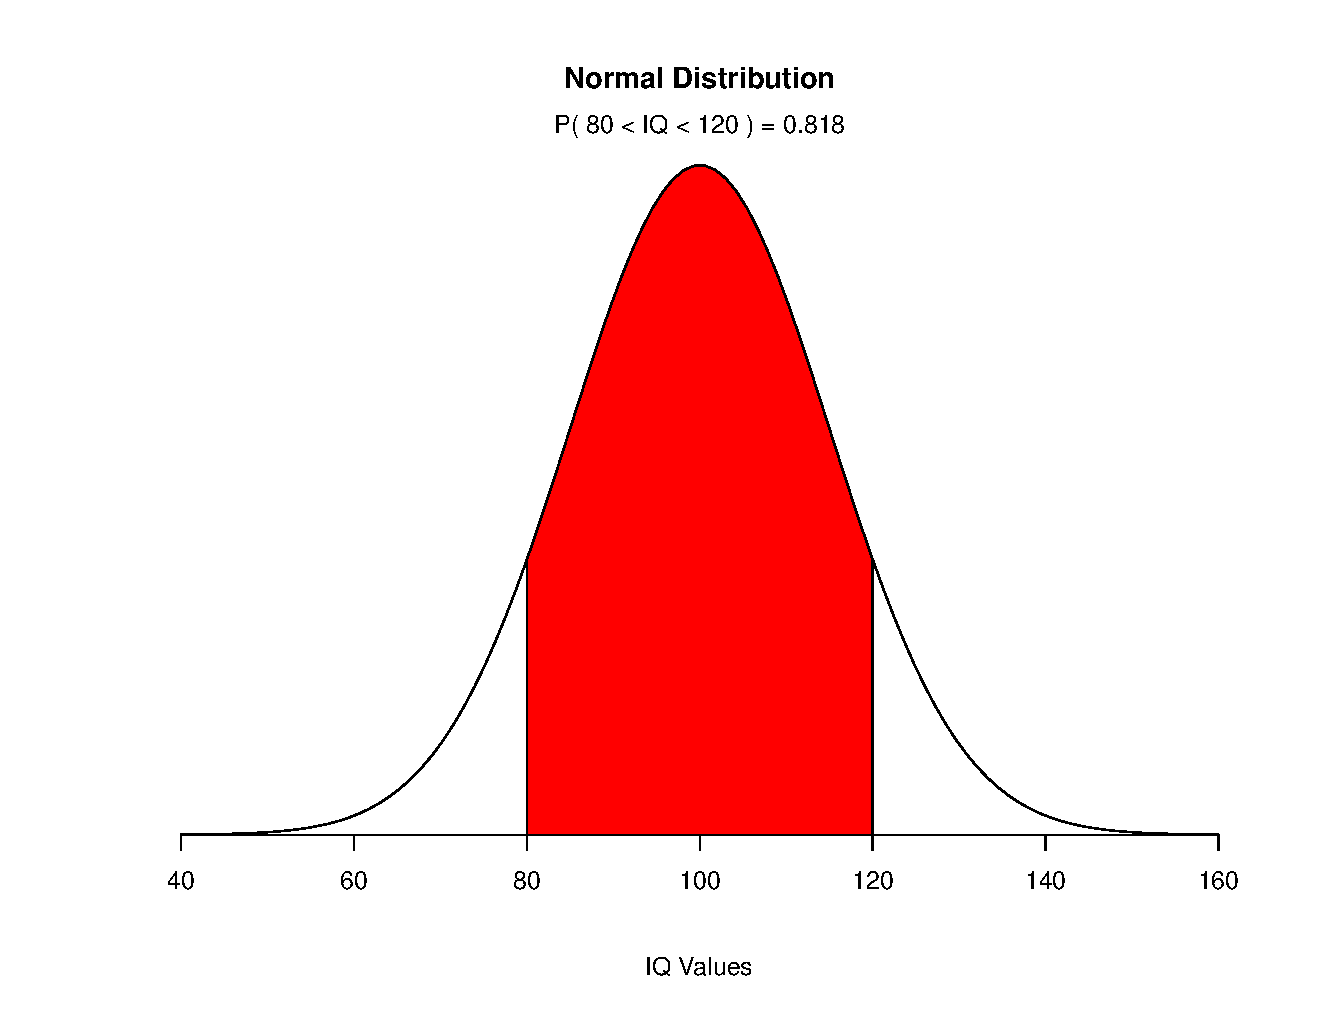
\includegraphics[width=0.4\textwidth]{img/normal}
\caption[Distribución normal]{Gráfica de una distribución normal. Fue creado usando el siguiente \href{https://www.statmethods.net/advgraphs/probability.html}{script en R}.}
\end{figure}
El caption y el resto del texto tienen la misma fuente
\end{frame}

\begin{frame}{Varias imágenes usando subfiguras}
\begin{figure}[htp]
 \centering
 \begin{subfigure}[b]{0.17\textwidth}
   
\includegraphics[width=\textwidth]{img/ambiente}
   \caption{Ambiental.}
 \label{fig:2a}
 \end{subfigure}
~
 \begin{subfigure}[b]{0.17\textwidth}
   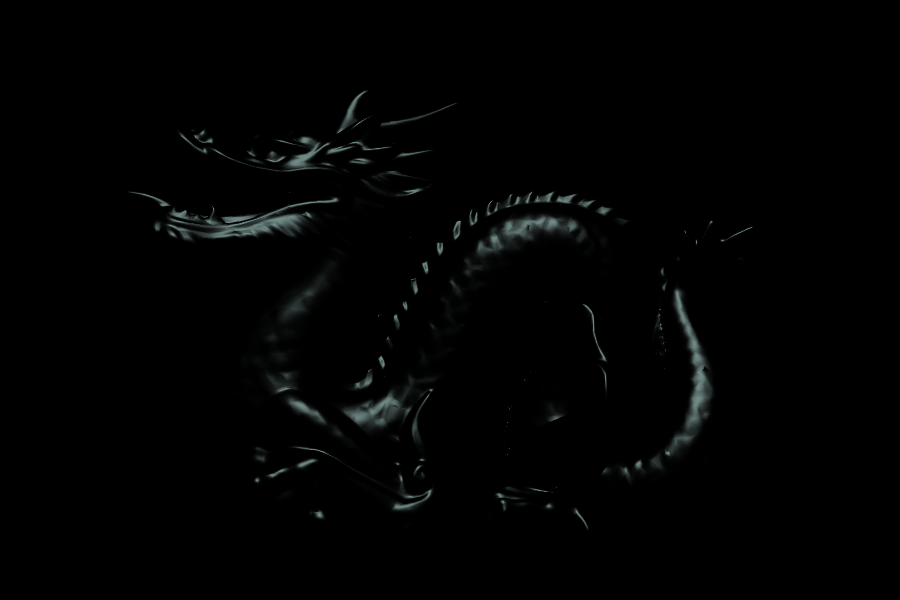
\includegraphics[width=\textwidth]{img/especular}
   \caption{Especular.}
   \label{fig:2b}
 \end{subfigure}
~
 \begin{subfigure}[b]{0.17\textwidth}
   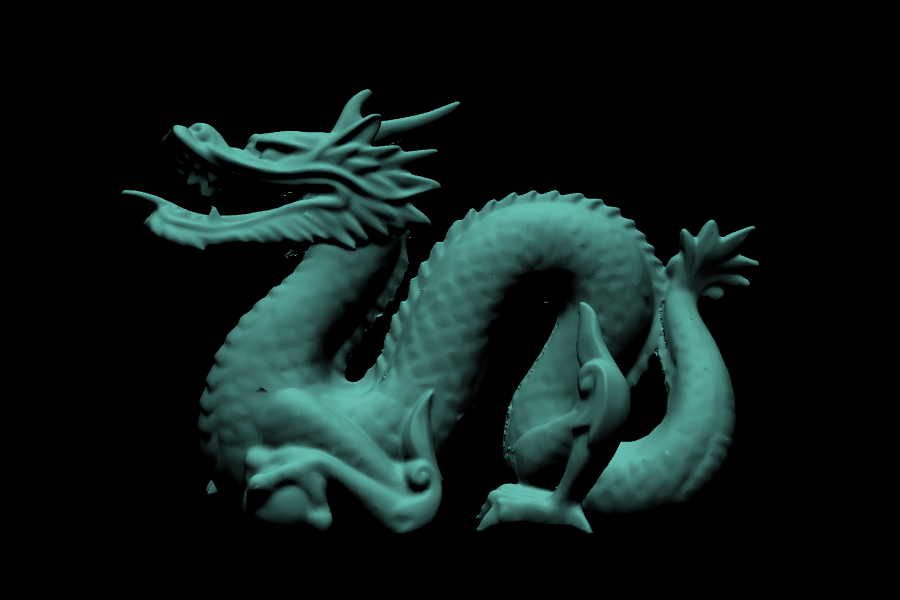
\includegraphics[width=\textwidth]{img/difuso}
   \caption{Difusa.}
   \label{fig:2c}
 \end{subfigure}
\\
 \begin{subfigure}[b]{0.22\textwidth}
   
\includegraphics[width=\textwidth]{img/completo}
   \caption{Modelo completo.}
   \label{fig:2d}
 \end{subfigure}
  \caption{Componentes del modelo de iluminación de Phong.}
  \label{fig:two}
\end{figure}
\end{frame}

\begin{frame}{Figura usando columnas}
\begin{columns}
\column[t]{0.5\textwidth}
 \begin{figure}[htb]
  \centering
  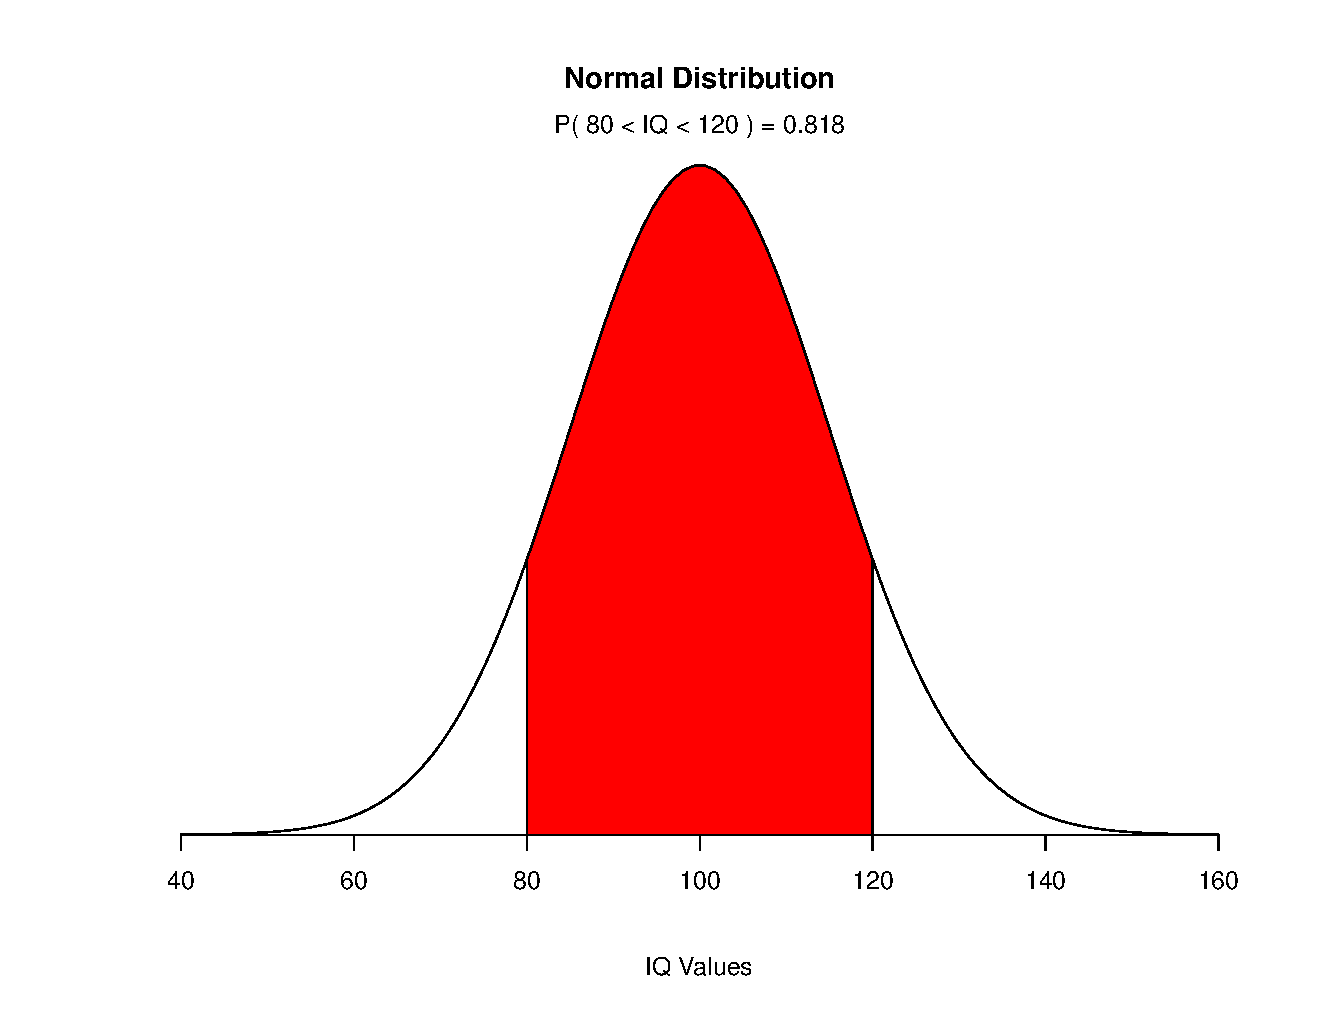
\includegraphics[width=0.7\textwidth]{img/normal}
\caption{Gráfica de una distribución normal.}
\end{figure}    
\column[t]{0.5\textwidth}
     Texto para describir la imagen
     \begin{enumerate}
         \item Se usan columnas
         \item La figura cambia de tamaño
         \item El caption puede apachurrase
     \end{enumerate}
\end{columns}
\end{frame}

\begin{frame}{Incluir tablas}
Este es un ejemplo de una tabla muy elegante.
Hace uso del paquete \href{https://ctan.org/pkg/booktabs}{booktabs} por que las tablas predeterminadas en \LaTeX{} se ven muy anticuadas.
Debes de consultar este \href{https://jdhao.github.io/2019/08/27/latex_table_with_booktabs/}{post} y leer esta \href{https://people.inf.ethz.ch/markusp/teaching/guides/guide-tables.pdf}{presentación} si vas a usar muchas tablas.
Este ejemplo también demuestra como poner \say{comillas}
\begin{table}[htb]
  \begin{center}
    \begin{tabular}{l | r r r r r}
      \toprule
      Source & \textbf{DF} & \textbf{SS} & \textbf{MS} & \textbf{F} & \textbf{P-value} \\
      \midrule
      \textbf{Model} & 2 & 0.00318564 & 0.00159282 & 7.72 & 0.0014 \\
      \textbf{Error} & 42 & 0.00866760 & 0.00020637 &  & \\
      \midrule
      \textbf{Total} & 44 & 0.01185324 &   &  & \\
      \bottomrule
    \end{tabular}
  \end{center}
\caption{Tabla ANOVA de un ejercicio imaginario}
\end{table}
\end{frame}

\section{Entornos de bloque}
\begin{frame}{Los entornos de bloque}
En esta diapositiva, el siguiente texto esta
\alert{resaltado} por que es importante.
Favor de no abusar.
\begin{block}{Bloque genérico}
    Texto dentro del bloque.
\end{block}

\begin{alertblock}{Bloque de Alerta}
    Texto dentro del bloque.
\end{alertblock}

\begin{exampleblock}{Bloque de Ejemplo}
    Texto dentro del bloque.
\end{exampleblock}   
\end{frame}

\section{Matemáticas}
\begin{frame}{Incluyendo matemáticas simples}
 \begin{equation}
 \label{eq:elipse}
 \frac{x^{2}}{a^{2}} + \frac{y^{2}}{b^{2}} = 1
 \end{equation}
 
  También se pueden insertar ecuaciones dentro de un párrafo, por ejemplo: $\forall x \in \mathbb{R}$.
\end{frame}

\begin{frame}{Resolviendo una integral}
Un ejemplo de cómo escribir una serie de pasos matemáticos usando el entorno: \texttt{align}.
Poner $*$ dentro del entorno te permite omitir los números
\begin{align*}
P\left(X \leq 3 \right) &= \int_{0}^{3} \frac{1}{25} y \,\mathrm{d}y \\
     &= \left. \frac{1}{25} \cdot \frac{1}{2} \, y^{2} \right|_0^3 \\
     &= \frac{1}{25} \left( \frac{1}{2} \, 9 - \frac{1}{2} \, 0 \right) =
     \frac{1}{25} \cdot \frac{9}{2} = \frac{9}{50} \approx 0.18 
\end{align*}
\end{frame}

\subsection{Ciencias de la computación}
\begin{frame}{Incluyendo un algoritmo}
\begin{algorithm}[H]
\renewcommand{\thealgorithm}{} % Quita el número del algoritmo en el caption
\caption{de Euclides}
\label{alg:euclid}
\begin{algorithmic}[1] % El número le dice al entrono desde que numero empezar a contar. Si le pones 0 omite los números
    \Procedure{Euclid}{$a,b$} \Comment{El g.c.d. de $a$ y $b$}
    \State $r\gets a \bmod b$
    \While{$r\not=0$} \Comment{Si $r = 0$, ya tenemos la respuesta}
        \State $a \gets b$
        \State $b \gets r$
        \State $r \gets a \bmod b$
    \EndWhile
    \State \textbf{return} $b$\Comment{$gcd = b$}
    \EndProcedure
\end{algorithmic}
\end{algorithm}

\end{frame}

\begin{frame}[fragile] % Usar minted requiere que uses opción fragile
\frametitle{Incluyendo código fuente}
\begin{listing}
\begin{minted}{cpp}
int main() {
  printf("hello, world");
  return 0;
}
\end{minted}
\caption{Un programa de ejemplo en C}
\end{listing}

Este es otro ejemplo de cómo incluir Python dentro de un párrafo: \mintinline{python}{print(x**2)}.

\end{frame}

\begin{frame}[fragile] % Usar minted requiere que uses opción fragile
\frametitle{Incluyendo código fuente desde un archivo}
\begin{listing}
\inputminted[
  firstline=54, % Si omites estos dos parámetros se usa todo el archivo
  lastline=68
  ]{cpp}{src/GccTest.cpp}
  \caption{Una implementación defectuosa de \textenglish{insertion sort}}\label{lst:example}
\end{listing}
\end{frame}


\end{document}
